\documentclass[11pt]{article}
\usepackage[margin=1in]{geometry}
\usepackage{amsmath,amssymb,amsthm}
\usepackage{graphicx}
\usepackage[T1]{fontenc}
\usepackage[utf8]{inputenc}
\usepackage{lmodern}
\usepackage[hidelinks]{hyperref}

\newtheorem{theorem}{Theorem}
\newtheorem{lemma}[theorem]{Lemma}
\newcommand{\WC}{\operatorname{WC}}
\newcommand{\PC}{\operatorname{PC}_{w^*,w}}

\title{Full Solution of Two General-Compact Converse Problems\\
for Weak-Star-to-Weak Points of Continuity}
\author{Run \texttt{fa\_banach\_001}, agent \texttt{agent\_lane\_08}}
\date{9 August 2026}

\begin{document}
\maketitle

\section*{Status and source questions}

\textbf{Status: full solution, likely valid, pending human review.}

Let $\Omega$ be nonempty compact Hausdorff and $X$ a nonzero Banach space.  Write
$\WC(\Omega,X)$ for the Banach space of bounded weakly continuous maps
$\Omega\to X$, with the supremum norm.  A functional $x^*\in B_{E^*}$ is a
\emph{weak-star-to-weak point of continuity} (abbreviated $w^*$-$w$ PC) when
the identity
\[
  (B_{E^*},w^*)\longrightarrow (B_{E^*},w)
\]
is continuous at $x^*$.

The source works under the standing convention that $\Omega$ is infinite.
Theorems 3.4 and 4.1 of Dwivedi \cite{source} prove necessary atomic
descriptions of the $w^*$-$w$ PCs in the dual balls of $C(\Omega,X)$ and
$\WC(\Omega,X)$, respectively.  On PDF pages 15--16 the paper asks:

\begin{quote}
\textbf{Question 4.6.} For a general compact Hausdorff space $\Omega$, is the
converse of Theorem 3.4 true?

\textbf{Question 4.7.} For a general compact Hausdorff space $\Omega$, is the
converse of Theorem 4.1 true?
\end{quote}

The source establishes both converses under extremal disconnectedness.  We
prove that this topological assumption is unnecessary.

\begin{figure}[ht]
  \centering
  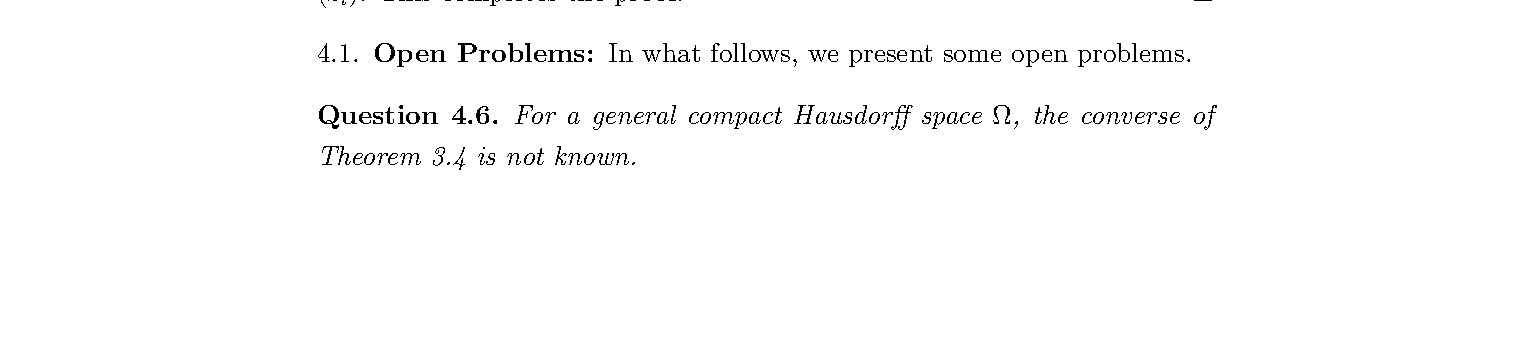
\includegraphics[width=\textwidth]{figures/open_problem_q46.png}
  \caption{Question 4.6 on source PDF page 15.}
\end{figure}

\begin{figure}[ht]
  \centering
  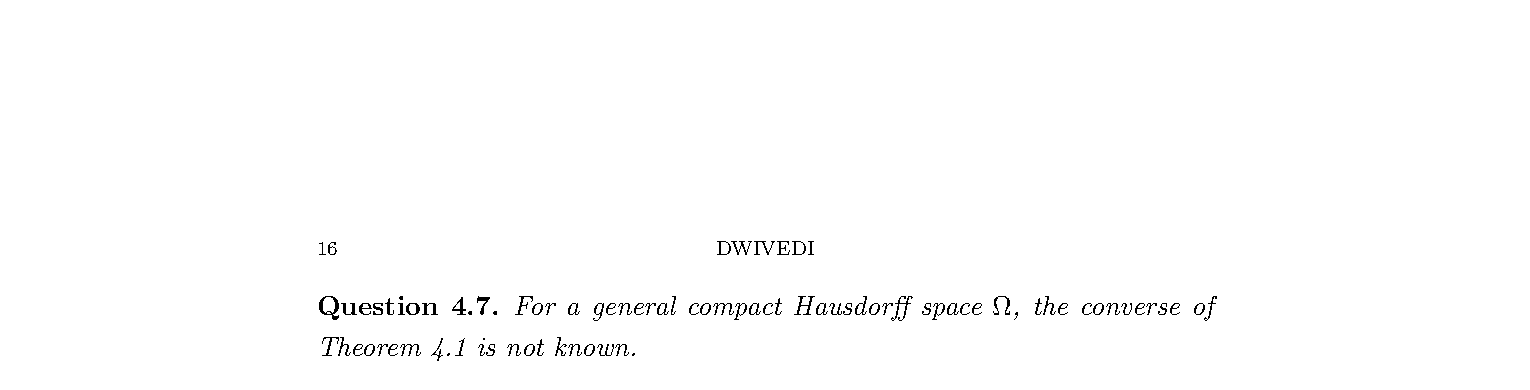
\includegraphics[width=\textwidth]{figures/open_problem_q47.png}
  \caption{Question 4.7 on source PDF page 16.}
\end{figure}

\section*{Proof intuition}

All relevant functionals live on isolated points.  If $I$ is the set of
isolated points of $\Omega$, then zero extension identifies $c_0(I,X)$ with a
subspace of both ambient function spaces.  A pointwise three-ball argument
shows that this subspace is always an $M$-ideal; density of $I$ and clopenness
of $\overline I$ are not needed.

On the dual $\ell_1(I,X^*)$, coordinatewise $w^*$ convergence by itself is not
enough for weak convergence.  The decisive extra fact is that the coordinate
norms of the proposed limit add up to the entire unit norm.  Lower
semicontinuity then forces convergence of each coordinate norm and uniform
smallness of the tails.  The coordinate PC hypothesis handles every finite
head, and the tail bound finishes the weak-convergence proof.  The standard
$M$-ideal lifting mechanism then transfers the PC to either ambient dual.
For completeness, the finite-space edge case is separated in the final
theorem: when both $\Omega$ is finite and $X$ is reflexive, the ambient space
is reflexive and every point of its dual ball is a PC.

\section*{The isolated-coordinate $M$-ideal}

We use the standard three-ball characterization of $M$-ideals
\cite[Chapter I]{hww}.

\begin{lemma}[isolated-coordinate lemma]\label{lem:mideal}
Let $S$ be a set, let $I\subseteq S$, and let $E$ be a closed linear subspace
of $\ell_\infty(S,X)$ which contains the zero extensions of $c_0(I,X)$.  Then
that copy of $c_0(I,X)$ is an $M$-ideal in $E$.
\end{lemma}

\begin{proof}
Put $Y=c_0(I,X)$, extended by zero on $S\setminus I$.  Take
$z\in B_E$, $y_1,y_2,y_3\in B_Y$, and $\varepsilon>0$.  There is a finite
$F\subseteq I$ such that
\[
  \lVert y_j(i)\rVert<\varepsilon
  \qquad(i\in I\setminus F,\ 1\leq j\leq 3).
\]
Define $y\in Y$ by $y(i)=z(i)$ for $i\in F$ and $y(s)=0$ otherwise.  For
$s\in F$,
\[
  (z+y_j-y)(s)=y_j(s),
\]
so its norm is at most one.  For $s\in I\setminus F$ its norm is at most
$1+\varepsilon$, and for $s\in S\setminus I$ it equals $\lVert z(s)\rVert$.
Consequently
\[
  \lVert z+y_j-y\rVert\leq 1+\varepsilon
  \qquad(1\leq j\leq3).
\]
This is the three-ball property, hence $Y$ is an $M$-ideal in $E$.
\end{proof}

If $I$ is the set of isolated points of a compact Hausdorff space $\Omega$,
zero extension maps $c_0(I,X)$ into $C(\Omega,X)$.  Indeed, for $u\in c_0(I,X)$
and $\varepsilon>0$, the set
$\{i\in I:\lVert u(i)\rVert\geq\varepsilon\}$ is finite and clopen in
$\Omega$; this proves continuity at every point outside $I$.  In particular,
the zero extensions also belong to $\WC(\Omega,X)$.  Lemma
\ref{lem:mideal} therefore applies to both ambient spaces.

\section*{Atomic PCs in the $\ell_1$-sum}

\begin{lemma}[full-mass atomic PC]\label{lem:l1}
Let $J\subseteq I$ be nonempty, finite or countable.  Let
$(x_i^*)_{i\in J}\subseteq S(X^*)$ consist of $w^*$-$w$ PCs of
$B_{X^*}$, and let $\alpha_i>0$ with $\sum_{i\in J}\alpha_i=1$.  Regard
\[
  \lambda=(\alpha_i x_i^*)_{i\in J}
\]
as an element of $B_{\ell_1(I,X^*)}$ by putting zero in the other coordinates.
Then $\lambda$ is a $w^*$-$w$ PC of
$B_{c_0(I,X)^*}=B_{\ell_1(I,X^*)}$.
\end{lemma}

\begin{proof}
Let $u_\gamma=(u_{\gamma,i}^*)_{i\in I}$ be a net in
$B_{\ell_1(I,X^*)}$ converging $w^*$ to $\lambda$.  For every $i\in J$,
testing against the $i$th coordinate copy of $X$ gives
\[
  u_{\gamma,i}^*\xrightarrow{w^*}\alpha_i x_i^*.
\]
For each finite $F\subseteq J$, weak-star lower semicontinuity of the norm
gives
\begin{equation}\label{eq:lsc}
  \liminf_\gamma\sum_{i\in F}\lVert u_{\gamma,i}^*\rVert
  \geq \sum_{i\in F}\alpha_i.
\end{equation}

Fix $i\in J$.  The one-coordinate case of \eqref{eq:lsc} gives the lower
bound for $\lVert u_{\gamma,i}^*\rVert$.  If $G$ is any finite subset of
$J\setminus\{i\}$, then
\[
  \lVert u_{\gamma,i}^*\rVert
  \leq 1-\sum_{j\in G}\lVert u_{\gamma,j}^*\rVert.
\]
Taking the upper limit and then finite $G$ whose $\alpha$-mass tends to
$1-\alpha_i$ yields
\[
  \lVert u_{\gamma,i}^*\rVert\longrightarrow\alpha_i.
\]
Thus, eventually normalizing the $i$th coordinate gives
\[
  \frac{u_{\gamma,i}^*}{\lVert u_{\gamma,i}^*\rVert}
  \xrightarrow{w^*}x_i^*.
\]
The PC hypothesis on $x_i^*$ upgrades this to weak convergence, so
$u_{\gamma,i}^*\to\alpha_i x_i^*$ weakly for every $i\in J$.

It remains to make the convergence uniform over the coordinates.  Given
$\eta>0$, choose finite $F\subseteq J$ with
$\sum_{i\in F}\alpha_i>1-\eta$.  Equation \eqref{eq:lsc} implies that,
eventually,
\[
  \sum_{i\notin F}\lVert u_{\gamma,i}^*\rVert<2\eta,
  \qquad
  \sum_{i\notin F}\alpha_i<\eta.
\]
Now take any $(x_i^{**})_{i\in I}\in\ell_\infty(I,X^{**})$.  The sum over
$F$ converges by coordinatewise weak convergence, while the two tails have
absolute value at most
$3\eta\sup_i\lVert x_i^{**}\rVert$.  Since $\eta$ is arbitrary,
$u_\gamma\to\lambda$ weakly in $\ell_1(I,X^*)$.
\end{proof}

\section*{Lifting through an $M$-ideal}

For completeness we record the short lifting step, also appearing as Lemma
3.1 of the source via \cite[Theorem 6.2]{dmr}.

\begin{lemma}[PC lifting]\label{lem:lift}
If $Y$ is an $M$-ideal in $E$, then a $w^*$-$w$ PC
$\lambda\in S(Y^*)$, viewed in the canonical $L$-summand of $E^*$, is a
$w^*$-$w$ PC of $B_{E^*}$.
\end{lemma}

\begin{proof}
Write $E^*=Y^\perp\oplus_1Y^\#$, where $Y^\#$ is the canonical copy of
$Y^*$.  Suppose $a_\gamma+b_\gamma\in B_{E^*}$ converges $w^*$ to
$\lambda\in Y^\#$.  Restriction to $Y$ shows that $b_\gamma\to\lambda$
$w^*$ in $B_{Y^*}$, hence weakly by the PC property.  Moreover,
\[
  1=\lVert\lambda\rVert
  \leq\liminf_\gamma\lVert b_\gamma\rVert,
  \qquad
  \lVert a_\gamma\rVert+\lVert b_\gamma\rVert\leq1,
\]
so $\lVert a_\gamma\rVert\to0$.  It follows that
$a_\gamma+b_\gamma\to\lambda$ weakly in $E^*$.
\end{proof}

\section*{Full classification}

\begin{theorem}\label{thm:main}
Let $\Omega$ be a nonempty compact Hausdorff space, let $X$ be a nonzero
Banach space, and let $E$ be either $C(\Omega,X)$ or $\WC(\Omega,X)$.

If $\Omega$ is finite and $X$ is reflexive, every point of $B_{E^*}$ is a
$w^*$-$w$ PC.  In every other case, a functional $\Lambda\in B_{E^*}$ is a
$w^*$-$w$ PC if and only if it has the canonical form, for a nonempty finite
or countable index set $J$,
\begin{equation}\label{eq:canonical}
  \Lambda=\sum_{n\in J}
  \alpha_n\,\delta_{\omega_n}\otimes x_n^*,
\end{equation}
where the $\omega_n$ are pairwise distinct isolated points of $\Omega$,
$\alpha_n>0$, $\sum_n\alpha_n=1$, and every
$x_n^*\in S(X^*)$ is a $w^*$-$w$ PC of $B_{X^*}$.
\end{theorem}

\begin{proof}
If $\Omega$ is finite and $X$ is reflexive, then
$E=\ell_\infty(\Omega,X)$ is reflexive, so the weak-star and weak topologies
coincide on all of $B_{E^*}$.

We next prove necessity outside this exceptional case.  For infinite
$\Omega$, it is Theorem 3.4 of \cite{source} for $E=C(\Omega,X)$ and Theorem
4.1 there for $E=\WC(\Omega,X)$.  Suppose instead that $\Omega$ is finite and
$X$ is nonreflexive.  Then $E=\ell_\infty(\Omega,X)$ is nonreflexive.  A
$w^*$-$w$ PC $u^*\in B_{E^*}$ must have norm one: otherwise, using the norm
slack at $u^*$, continuity there would make every bounded weak-star-null net
weakly null after scaling.  It would follow that weak-star convergence implies
weak convergence on $B_{E^*}$, making $B_{E^*}$ weakly compact and $E$
reflexive, a contradiction.  Write
$u^*=(u_\omega^*)_{\omega\in\Omega}\in\ell_1(\Omega,X^*)$.  If
$u_\omega^*\ne0$, replace its coordinate by
$\lVert u_\omega^*\rVert v_\gamma^*$ for an arbitrary net
$v_\gamma^*\in B_{X^*}$ converging weak-star to
$u_\omega^*/\lVert u_\omega^*\rVert$.  The resulting net remains in
$B_{E^*}$ and converges weak-star to $u^*$; the PC property and the coordinate
projection therefore show that $v_\gamma^*$ converges weakly.  Thus every
normalized nonzero coordinate is a PC, which is exactly the stated canonical
form.

For sufficiency, let $I$ be the set of isolated points and let
$Y=c_0(I,X)$, extended by zero.  Lemma \ref{lem:mideal} says that $Y$ is an
$M$-ideal in either choice of $E$.  Under
$Y^*=\ell_1(I,X^*)$, the restriction of \eqref{eq:canonical} is exactly the
full-mass atomic functional of Lemma \ref{lem:l1}; hence it is a $w^*$-$w$ PC
of $B_{Y^*}$.  Its canonical extension in the $L$-summand of $E^*$ is
precisely \eqref{eq:canonical}.  Lemma \ref{lem:lift} completes the proof.
\end{proof}

Thus both Questions 4.6 and 4.7 have affirmative answers.  In particular, the
source's topological hypothesis is unnecessary.  The extra finite-space clause
above supplies the literal all-compact classification beyond the source's
standing infinite-space convention.

\section*{Verification and limitations}

The proof uses nets throughout.  It allows uncountable $I$: only the countable
support of \eqref{eq:canonical} enters the finite-head argument, while the
tail estimate controls every coordinate outside a chosen finite subset.
Pairwise distinct support points are part of the canonical support
decomposition.  If a display repeats a point, its atoms must first be combined,
and the normalized combined coordinate must satisfy the PC hypothesis.

The three-ball estimate was checked in its three pointwise regimes: on the
finite copied set, on the remaining isolated points, and off the isolated set.
The finite/reflexive exception was checked separately rather than being hidden
inside the source's infinite-space convention.  No computational verification
is relevant.

This packet does not address Questions 4.8 or 4.9 of the source.

\section*{Bounded novelty search}

On 9 August 2026 we searched the run's registry, solution, attempt, and
proof-gap indexes for arXiv:2604.09133 and the core terms.  Web searches used
the exact paper title, the quoted converse formulations, $w^*$-$w$ PC terms
for $C(K,X)$ and $\WC(K,X)$, and the $c_0(I,X)$/$M$-ideal mechanism.  They
found the source preprint and older background literature, including
\cite{dmr}, but no separate paper explicitly answering either general
converse.  This supports, but does not guarantee, novelty.

\section*{Human-review focus}

The three decisive checks are: (i) applying the standard three-ball
characterization in Lemma \ref{lem:mideal}; (ii) the norm-saturation and tail
argument in Lemma \ref{lem:l1}; and (iii) identifying the atomic functional
with the canonical $L$-summand extension in Lemma \ref{lem:lift}.

\begin{thebibliography}{9}

\bibitem{source}
S. Dwivedi,
\emph{An extension of Phelps theorem to spaces of vector-valued functions},
arXiv:2604.09133v1 (2026),
\url{https://arxiv.org/abs/2604.09133}.

\bibitem{dmr}
S. Daptari, V. Montesinos, and T. S. S. R. K. Rao,
\emph{A study of weak$^*$-weak points of continuity in the unit ball of dual
spaces}, Rev. R. Acad. Cienc. Exactas F\'is. Nat. Ser. A Mat. 119 (2025), 82;
arXiv:2506.08458,
\url{https://arxiv.org/abs/2506.08458}.

\bibitem{hww}
P. Harmand, D. Werner, and W. Werner,
\emph{$M$-Ideals in Banach Spaces and Banach Algebras},
Lecture Notes in Mathematics 1547, Springer, 1993.

\end{thebibliography}

\end{document}
